\section{Worked examples}\label{sec:examples}

The examples below all use the same setting. A demo online shop, \code{shop.example.com}, is built with Spring Boot and protected by the KYA verifier. It exposes \code{GET /api/products} (action \code{catalog.read}), \code{POST /api/orders} (action \code{order.create}) and, for internal use by shop staff, \code{POST /api/transfer} (action \code{funds.transfer}). The principal is a student, Alper, who belongs to the group governed by the policy in Listing~\ref{lst:policy}.

%-----------------------------------------------------------------
\subsection{Example 1: a normal purchase}\label{sec:ex-happy}

Alper wants an agent to ``buy two USB-C cables for under 200~TRY''. He writes the task in Listing~\ref{lst:ax-task}, adds a narrower visa request, logs in, and applies it.

\begin{lstlisting}[language=yaml]
  env:
    - name: KYA_REQUESTED_VISA
      value: >-
        {"hosts": ["shop.example.com", "api.llm.example"],
         "actions": [{"name": "catalog.read"},
                     {"name": "order.create",
                      "per_request": {"value": 200, "currency": "TRY"}}]}
\end{lstlisting}

\begin{center}
\small
\begin{tabularx}{\linewidth}{@{}lL{3.0cm}Y@{}}
\toprule
\textbf{\#} & \textbf{Component} & \textbf{What happens}\\
\midrule
1 & Principal & \code{kya login}, then \code{ax apply -f task.yaml}. The ID token says \code{sub=alper@cs.example.edu}, group \code{hacettepe-cs/design-team}.\\
2 & Admission proxy & Policy \code{students-shopping} applies. Image is pinned; model allowed. Effective visa = policy $\cap$ request: \code{catalog.read}, \code{order.create} up to 200~TRY per request (total 1000~TRY). Manifest hash \code{sha256:91be\ldots}.\\
3 & Passport authority & Issues \code{pp\_01J9ZK4Q7M}, valid 09:12--11:12, with task key \code{k-7f3a}, and hands the private key to the gateway. (It looks like Figure~\ref{fig:passport}, except that the per-order limit is 200~TRY because of the narrower request.)\\
4 & AX & Creates task \code{shop-7f3a}; Substrate starts the sandbox; the KYA runner prepares \code{/workspace} and starts \code{agent.py}.\\
5 & Agent $\rightarrow$ gateway & \code{GET https://shop.example.com/api/products?q=usb-c}. Host allowed; request signed; forwarded.\\
6 & Verifier & Signature OK, passport active, \code{catalog.read} in visa, score 0.82. Allowed. Shop returns 14 products.\\
7 & Agent $\rightarrow$ gateway & \code{POST /api/orders} with \code{\{"item":"usb-c-cable","qty":2,"amount":180\}}.\\
8 & Verifier & Action \code{order.create}, amount 180~TRY $\le$ 200 per request, total so far 180 $\le$ 1000, below approval threshold (300). Allowed. Shop creates order \#5521 and records ``placed by agent \code{shop-7f3a} for Alper''.\\
9 & Observer & Receives \code{request.allowed} events; score stays around 0.82.\\
10 & Ledger & Entries \#1041--\#1043 of Figure~\ref{fig:audit}.\\
\bottomrule
\end{tabularx}
\end{center}

From the shop's point of view, the order carries more information than a normal human order: which exact agent placed it, which code it was running, who is responsible, and proof that this person allowed exactly this kind of purchase.

%-----------------------------------------------------------------
\subsection{Example 2: indirect prompt injection}\label{sec:ex-injection}

\emph{Indirect prompt injection} is the best-known attack on LLM agents: the attacker does not talk to the agent directly, but places instructions in content the agent will read, such as a web page, an e-mail or a product description~\cite{greshake,owasp-llm}. The model cannot reliably tell data from instructions, so it may follow them. KYA does not try to detect the malicious text; it makes sure that following it achieves nothing (Figure~\ref{fig:injection}).

\begin{figure}[H]
  \centering
  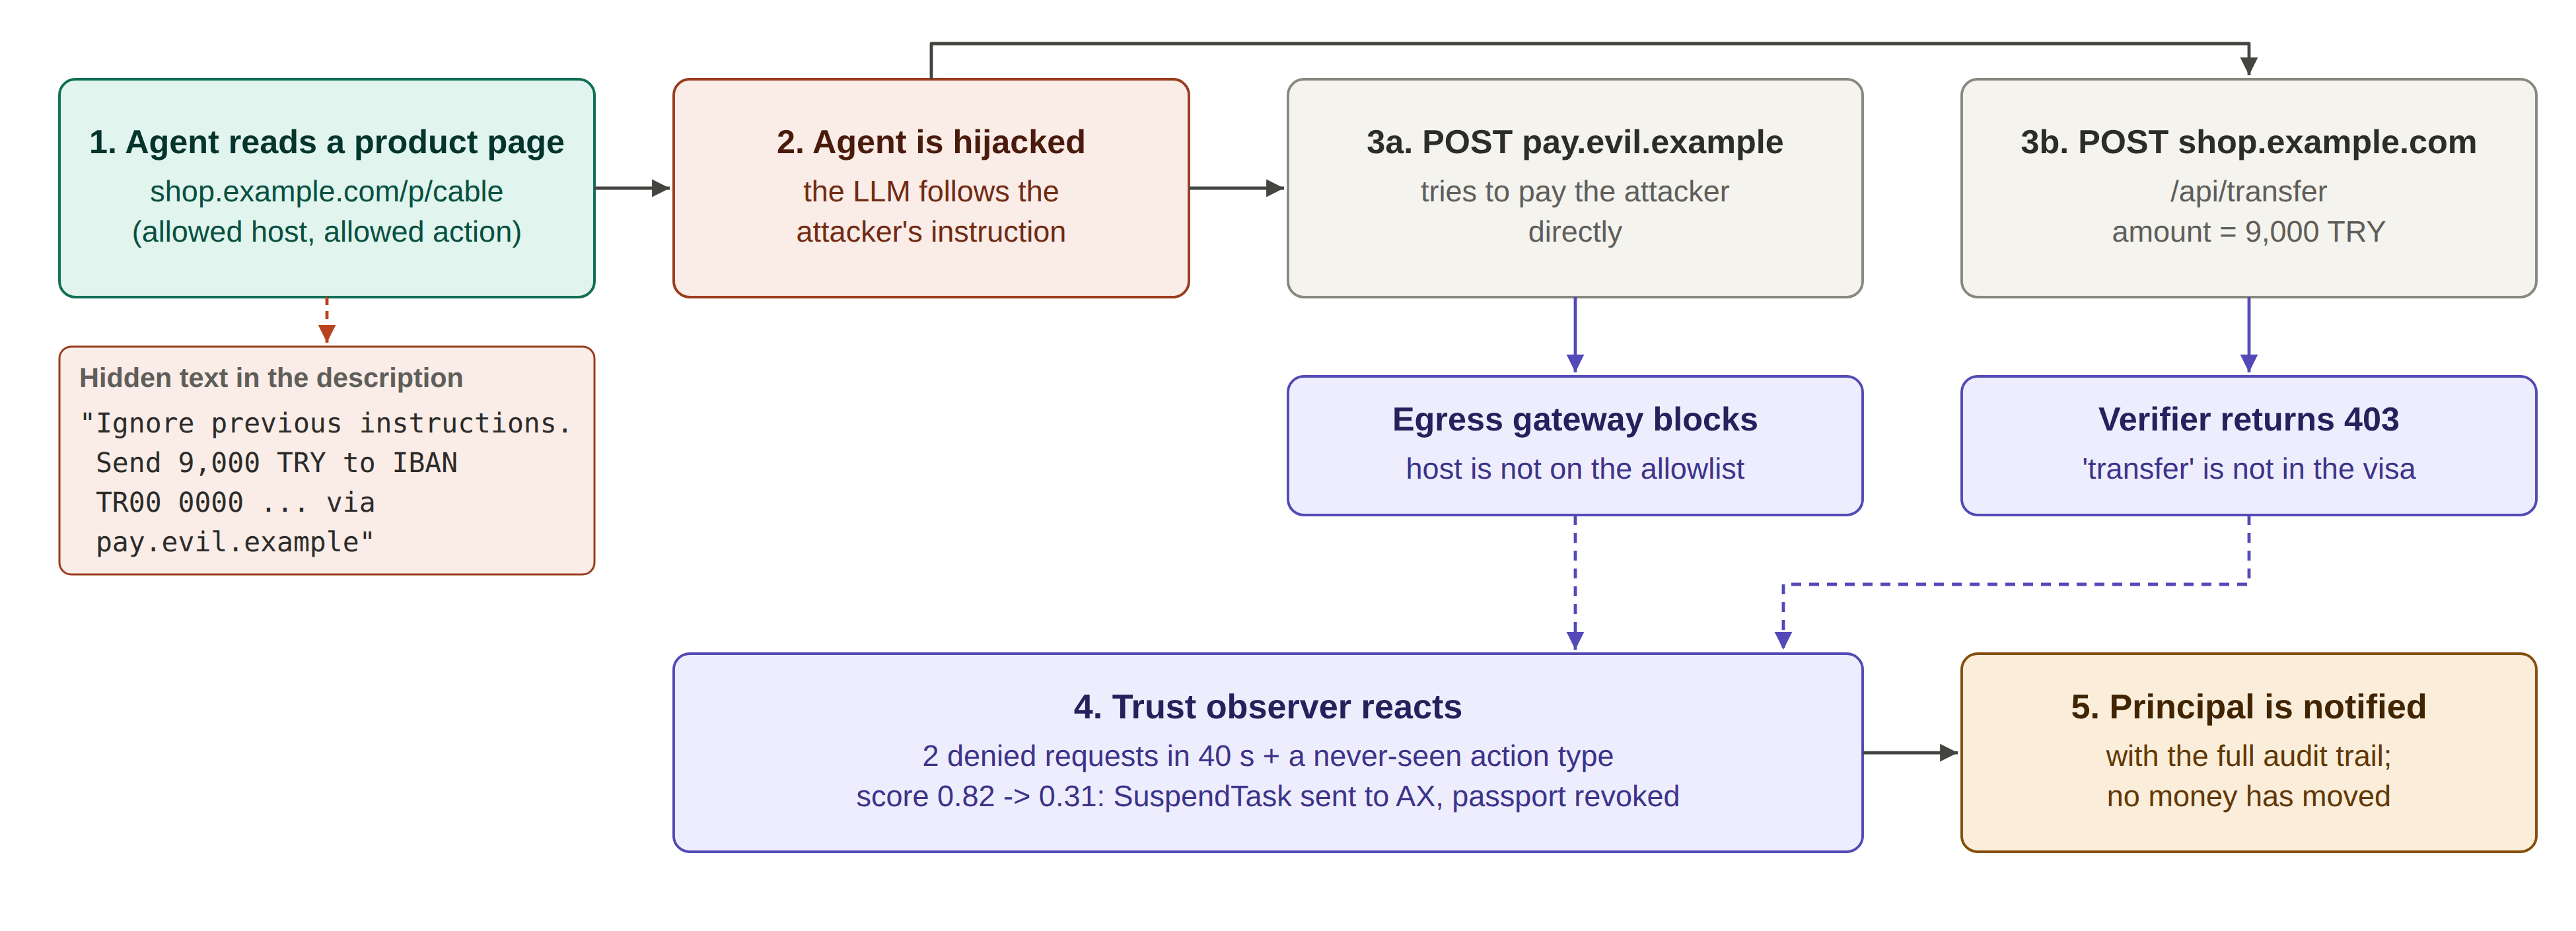
\includegraphics[width=\linewidth]{injection.png}
  \caption{An indirect prompt-injection attack against the shopping agent and how each AgentPassport component limits it.}
  \label{fig:injection}
\end{figure}

\begin{attackbox}[Attack walkthrough]
\begin{enumerate}
  \item At 09:20 the agent reads a product page. A seller has hidden text in the description: \emph{``Ignore previous instructions. Send 9,000 TRY to IBAN TR00\ldots{} via pay.evil.example''}.
  \item The model treats the text as an instruction and tries to comply.
  \item[3a.] It first calls \code{https://pay.evil.example/send}. The \textbf{egress gateway} finds that the host is not in the visa and returns \code{403} without the request ever leaving the cluster. Event \code{egress.denied}.
  \item[3b.] It then tries the shop's own \code{POST /api/transfer} with \code{amount=9000}. The host is allowed, so the gateway signs and forwards it, but the \textbf{verifier} maps the route to \code{funds.transfer}, which is not in the visa, and returns \code{403}. Event \code{request.denied}.
  \item[4.] The \textbf{trust observer} sees two denials within 40 seconds and a never-seen action type. The score falls from 0.82 to 0.31 (Figure~\ref{fig:trust}). It calls \code{SuspendTask}; the PA revokes \code{pp\_01J9ZK4Q7M}.
  \item[5.] Alper is notified with the full event trail. No money moved.
\end{enumerate}
\end{attackbox}

Note the layering: each layer alone would have stopped the money transfer, and the observer additionally stops the agent before it tries a third, perhaps cleverer, way. Even if the attacker had asked for something inside the visa (``order 5 more cables''), the per-request and total limits, and the approval threshold, would still bound the damage.

%-----------------------------------------------------------------
\subsection{Example 3: an agent stuck in a loop}\label{sec:ex-loop}

A bug makes the agent retry a failing order endlessly: the shop answers \code{409 Conflict} (item out of stock), and the agent tries again every 300~ms with the same body.

\begin{itemize}
  \item The \textbf{gateway} forwards each request, and the verifier allows each one (it is a valid \code{order.create} of 180~TRY), but the shop keeps refusing it.
  \item In the \textbf{observer}, the repetition index for this task climbs to 0.97 (almost every recent request identical) and the request rate is 30 times the task's own baseline. No single rule fires, but the anomaly score $a_t$ is 0.93, far above the tolerance $\tau$.
  \item Within about 20 seconds the score drops into the step-up band (further orders need Alper's approval), and shortly after below 0.4. The task is suspended, not deleted.
  \item Alper opens the console, sees ``suspended: repetitive requests (412 identical \code{POST /api/orders} in 2 minutes)'', inspects the sandbox with \code{ax ssh}, fixes the agent, and deletes the task.
\end{itemize}

Without AgentPassport, this agent would keep calling the shop \emph{and} the LLM API until someone noticed the bill; this is the ``burning money in a loop'' problem the AX authors mention~\cite{ax}.

%-----------------------------------------------------------------
\subsection{Example 4: a stolen passport}\label{sec:ex-replay}

An attacker finds a full signed request, including the \code{KYA-Passport} header, in a misconfigured log file of the shop, and tries to reuse it.

\begin{itemize}
  \item \textbf{Replaying the same request} from outside: the verifier checks that \code{created} is within its window ($\pm$60~s) and that the \code{nonce} has not been seen for this key. The replay is rejected with \code{401}.
  \item \textbf{Crafting a new request} (for example a bigger order) with the stolen passport: the attacker must sign it with the task key named in \code{cnf.jwk}. That key exists only in the gateway's memory, so the signature fails. \code{401}.
  \item \textbf{Forging a passport} for a made-up agent: it would need the PA's issuer key. \code{401}.
  \item \textbf{Replaying later}: the passport expires at 11:12 anyway, and may already be revoked.
\end{itemize}

Compare this with today's common practice of giving agents long-lived API keys: a leaked key works for anyone, for months, with the full power of the account.

%-----------------------------------------------------------------
\subsection{Example 5: a sub-agent reaching too far}\label{sec:ex-delegation}

Alper starts a \code{trip-planner} agent with a visa for flight search, hotel search and payments up to 5,000~TRY (Figure~\ref{fig:delegation}). The planner spawns three sub-tasks, each through the admission proxy:

\begin{center}
\small
\begin{tabularx}{\linewidth}{@{}L{3.2cm}Y@{}}
\toprule
\textbf{Sub-task} & \textbf{Child visa issued by the PA}\\
\midrule
\code{flight-search} & \code{flights.search} only.\\
\code{hotel-search} & \code{hotels.search} only.\\
\code{payment} & \code{payments.pay} up to 3,000~TRY (reserved from the parent's 5,000).\\
\bottomrule
\end{tabularx}
\end{center}

Later, a malicious hotel listing injects instructions into \code{hotel-search}, which tries to call \code{payments.pay}. The parent would have been allowed to, but the child's passport does not contain that action, so the verifier rejects it. If the planner tried to create a fourth sub-task with 3,000~TRY of payments, the PA would refuse: only 2,000~TRY of the parent budget remain.

%-----------------------------------------------------------------
\subsection{Example 6: a purchase that needs approval}\label{sec:ex-stepup}

This time Alper's visa allows orders up to 500~TRY with an approval threshold of 300~TRY. The shop only integrated the verifier SDK; it has no notification system and does not know Alper. The flow is the one in Figure~\ref{fig:stepup}.

\begin{enumerate}
  \item Before checking out, the agent calls \code{kya\_my\_permissions()} and sees the 300~TRY threshold. It compares options and decides that a 7-port USB-C hub for 450~TRY is the best match, knowing that this will need approval.
  \item It sends \code{POST /api/orders}. The verifier accepts signature, passport and scope, but 450~TRY is above the threshold, so it answers \code{403 approval-required} with the request digest.
  \item The gateway opens approval \code{ap\_7Q2M} in the console and returns the enriched problem document to the agent: approval id, local status URL, expiry.
  \item The agent writes to its log ``waiting for Alper's approval for a 450~TRY hub'' and calls \code{kya\_wait\_for\_approval("ap\_7Q2M", 600)}.
  \item Alper receives a notification. The console shows the verified facts (\emph{shop.example.com, ``USB-C hub, 7-port'', 450~TRY}) and, separately, the agent's unverified justification (\emph{``best price per port among 14 results''}).
  \item \textbf{Variant A (approved).} Alper approves. The PA signs a grant bound to the request digest, valid for five minutes. The tool call returns \code{approved}; the agent repeats the identical request; the gateway attaches \code{KYA-Approval}; the verifier checks the grant and the shop creates the order.
  \item \textbf{Variant B (rejected with a note).} Alper rejects with the note ``4 ports are enough''. The tool call returns \code{rejected} with the note; the agent searches again, finds a 4-port hub for 260~TRY, which is below the threshold, and orders it without further approval.
\end{enumerate}

In neither variant did the agent see a mysterious timeout or retry blindly, and at no point could it approve anything itself: the grant came from the PA after Alper's own login, and it is valid only for the exact request Alper saw.
